\documentclass[11pt,twocolumn]{jarticle} %11pt が MS-Word の10.5pt 相当
\usepackage[a4paper,left=23mm,right=23mm,top=27mm,bottom=32mm]{geometry} 

\usepackage[dvipdfmx]{graphicx}
\usepackage{iit-en-sjis} %use iit-en-sjis if the body text is written English.
\usepackage{wrapfig}
\usepackage{algorithm, algpseudocode}
\usepackage{algorithmicx}
\usepackage{comment}
\usepackage{amsfonts}
\usepackage{amsmath}

\graphicspath{ {imgs/} }

\title{捕食者・獲物環境におけるマルチエージェントの分散型協調学習}
\etitle{Distributed Multi-Agent Cooperation Learning in Predator-Prey Environment}

\author{唐 \ \ 霄}
\eauthor{TANG Xiao}

\advisors{
\footnotesize
\begin{tabular}{ll}
 指導教員: & 延原 肇, 中内 靖, 星野 准一(知能機能工学域)\\
\end{tabular}
}
\eadvisors{
\scriptsize
\begin{tabular}{ll}
Supervised by: & Nobuhara Hajime, Yasushi Nakauchi and Junichi Hoshino (Division of Intelligent Interaction Technologies) \\
\end{tabular}
}

\authorheader{唐 \ 霄}
% use English name when you use the English style

\dateheader{2018年1月}

\abstract{
(Remain modification)
Research of Moving Target Search is ongoing recent years. There are some researches according to the problem of Multi-Agent pursuing a moving target, but few of them could be applied to real world. This research focused on this problem and proposed a speed-up method for real-time grid environment based on Cover Heuristic method. We use Map Abstraction to build map hierarchy which helps us do faster map search compared to previous method. Refinement is used for highly-abstracted route refining to successor original map. Finally, evaluation experiments are based on Benchmark maps and the result showed high efficiency of our proposed method.
}

\keywords{keyword-1, keyword-2, keyword-3, keyword-4, keyword-5, keyword-6}

\begin{document}

\maketitle
\thispagestyle{iitheader}
\section{Introduction}
Recently, AI arouse hot topics around the world, especially after the appearence of AlphaGo\cite{alphago}. DeepMind introduced their Go player which is called AlphaGo in 2015, it beat several human being's top professional players over the past two years. And AlphaGo evolved to become nearly unbeatable versions which are AlphaGo Master and AlphaGo Zero\cite{alphagozero}. AI not only contribute to the application of traditional sports, game is also a big area which studies are ongoing. DeepMind and Blizzard released StarCraft II platform as an AI research environment\cite{starcraft} for researchers around the world.\par

\begin{figure}[t]
 \begin{center}
  \includegraphics[width=5cm]{imgs/adversary_chasing.png}
  \caption{Predator-Prey(CHANGE)}
  \label{fig:adversaryChasing}
 \end{center}
\end{figure}

Deep Reinforcement Learning (DRL) is one of the technologies which support AI development. There are a lot of applications from game playing\cite{game} to robot controlling\cite{robot}. Also, Google applied Deep Learning to data center cooling by 40\%\cite{google} electric cost off. Healthcare and finance (REFERENCE paper) are the areas which are being researched and expected to have great impact to sociaty. However, despite the fact that DRL is successfully applied to many single-agent domain tasks, there are varianty of applications which are in multi-agent domain. These application needs multiple agents to evolve together to be capable of good communication or cooperation. For instance, multi-character controlling in game playing, multi-agent system in delivery system and so on.


One representative for multi-agent task is Predator-Prey\cite{maddpg}, showed in Fg.\ref{fig:adversaryChasing}. In this case, there are 3 predators, 1 prey and 2 landmarks (obstacles) in this map. Predators move with slower speed to chase the faster moving prey. For human being, the cooperation strategy of splitting up and surrounding is absolutely easy to understand and learn. Unfortunately, it is difficult for agent to learn. Although Traditional reinforcement learning such as Q-learning\cite{qlearning}, Policy Gradient\cite{pg} performs well and even better than human being in Atari Game\cite{ddpg}, it performs poorly in multi-agent domain. The reason why the successful RL methods using in single-agent domains could not acquire the same result in multi-agent domain is that along with mult-agent self-learning, the environment becomes non-stationary which force learning fail to convergence. \par

(CHANGE)
We have two problems in multi-agent task, one is that traditional RL methods can't solve multi-agent task because environment becomes non-stationary during learning, the second one is that random sampling batch data from experience replay may not be effcient enough for learning. In this work, we first introduce several prior works and related researches and explain why they failed in multi-agent domain. Then we will explain our proposed method - Distributed Multi-Agent Cooperation Algorithm besed on MADDPG algorithm\cite{maddpg} using prioritized batch data in solving Predator-Prey task. Experiments shows we achieve xx\% faster and xx times rewards comparing to MADDPG and DDPG.\par

\section{Background} 
In this section, we introduce our prior researches and problem definition of multi-agent markov decision process.
\subsection{Cover-hueristic Algorithm\cite{cover}}
As for prior research for solving Predator-Prey, I have proposed a cooperation searching algorithm towards this task. This method is based on map search using speed-up cover-heuristic \cite{cover-heuristic} (maxmizing Predator's moving area and minimizing prey's moving area) and accelarating search by map abstraction and refinement. However, this method performs well in small-size maps but poorly in big-size maps, the computational time is depends on the map size. A agent which could be called intelligent should have its own mind like human beings. This kind of AI is able to take actions based one its own policy.\par


\subsection{Reinforcement Learning and Multi-Agent Markov Decision Process}

Reinforcement Learning (RL) is method that agent learns to make decisions through interaction with environment. An agent interacts with environment and becomes able to alter its behaviour according to the reward it recieved from environment along with observing the consequences of its actions. \par

\begin{figure}[h]
 \begin{center}
  \includegraphics[width=8cm]{imgs/RL.PNG}
  \caption{
  Overview of RL.
  }
  \label{fig:rl}
 \end{center}
\end{figure}

In RL settings, agent is controlled by specific algorithm (machine learning). The action-learning loop is illustrated in Fg.\ref{fig:rl}. Assume we have a set of States from environment: $S \subseteq \mathbb{R}^n$ which describes possible configurations of environment, a set of Actions for agent: $A \subseteq \mathbb{R}^m$ which agent executes to interact with environment, and a set of Rewards: $R \subseteq \mathbb{R}$ which is the feedback for agent given by environment, where $m, n$ differs in different environment. At each timestep, the agent observes a state $s \in S$ and interacts with environment by taking an action $a \in A$. After agent takes an action, the environment and agent transition to a new state $s' \in S$. Then agent recieves an reward $r \in R$  as feedback. Agent has a policy $\pi$ which maps  a state to a action $\pi: S \rightarrow A$. The agent uses experience of state transition, a form of ($s$, $a$, $r$, $s'$). The goal of agent is to learn an optimal policy which maximizes the expected cumulative return. The challenge in RL is that agent needs to learn about the consequences of actions by trail and error. \par

RL could be described as a Markov Decision Process (MDP). In this work, we extend MDP from single-agent domain to multi-agent setting. The multi-agent MDP consists:
\begin{itemize}
  \item $n$ Agents, $n \in \mathbb{R}$
  \item A set of private observations $O$ from state. 
  \item A set of observations \{${o_1, o_2,\ldots, o_i\ldots, o_n}$\} $\subseteq O$ which describes each agent's private observation.
  \item A set of actions \{${a_1, a_2,\ldots, a_i,\ldots, a_n}$\} $\subseteq A$.
  \item A set of rewards \{${r_1, r_2,\ldots, r_i,\ldots, r_n}$\} $\subseteq R$, agents recieves rewards from environment after execution actions.
  \item Policy $\pi_i$ of agent $i$: $\pi_i: O \rightarrow A$ which maps one observation to one action.
\end{itemize}
The return from start of agent $i$ is defined as the sum of futuren reward which could be represented as, 
$$ R_i = \sum_{t=0}^{T}(\gamma^t r^{t}_i) $$
where $t$ is timestep and $T$ is the terminal timestep, gamma is the discounted factor $\gamma \in [0, 1]$ and $r^{t}_i$ is the reward of agent $i$ at $t$ timestep.

\section{Related Works}

Currently, there are three approaches to solve MDP problems: value-based method, policy-based method and actor-critic method. We will discuss these methods about their advantages and drawbacks in solve multi-agent domain problems.

\subsection{Value-based Method}

Value-based method is based on estimating the expected return of being given a state. The state-value function is the expected return when starting in state $s$ and following policy $\pi$ henceforth: 

\begin{equation}
V^\pi(s) = \mathbb{E}[R] = \mathbb{E}[\sum_{t=0}^{\infty}\gamma^t r_t | s_0 = s].
\end{equation}

When we have the optimal policy, $\pi$ b ecomes $\pi^*$ which has maximal value of $V^\pi(s)$. However, value function can not provide us transitions for agent to learn. Therefore, action-value function $Q^\pi(s, a)$ was constructed:
\begin{equation}
Q^\pi(s, a) = \mathbb{E}[R] = \mathbb{E}[\sum_{t=0}^{\infty}\gamma^t r_t | s_0 = s, a_0 = a]. 
\end{equation}

action-value function describes the expected return for selecting action $a$ in state $s$ and then following policy $\pi$. An optimal action value function $Q^*(s, a)$ could be found by choosing maximal $Q$ value with action $a$. Under optimal policy, $V^\pi(s) = \arg\max_a{Q^\pi(s, a)}$.

\subsubsection{Q-learning\cite{qlearning}}

Q-learning is one of famous algorithms in RL. We update action-value function using a Bellman equation: 
\begin{equation}
Q^\pi(s_t, a_t) = \mathbb{E}[r_{t} + \gamma Q^\pi(s_{t+1}, \pi(s_{t+1}))].  
\end{equation}
which means we can use represent current Q value with next Q value.
\begin{equation}
Q^\pi(s_t, a_t) \leftarrow Q^\pi(s_t, a_t) + \alpha\delta.  
\end{equation}
where $t$ is timestep, $\alpha$ is learning rate and $\delta$ is the Temporal Difference (TD) error:
\begin{equation}
\delta = y - Q^\pi(s_t, a_t)
\end{equation}
We can see that $Q^\pi$ can be improved by \textsl{bootstrapping}.\par 
Q-learning is an off-policy algorithm, because $Q^\pi$ is updated by transitions that were not generated by derived policy where 
\begin{equation}
y = r_t + \gamma\max Q^\pi(s_{t+1}, a)
\end{equation}
which is used to approximate $Q^*$.

\subsubsection{Deep Q-Network\cite{dqn}}

Deep Q-Network (DQN) is the extended version of Q-learning using deep learning. It uses a deep neural network to work as the Q value function. 

\begin{equation} \label{eq:dqn-loss}
L(\theta) = \mathbb{E}_{s,a,r,s'}[y - Q(s, a|\theta))],  
\end{equation}
$$where y = r + \gamma\max \bar{Q}^*(s', a'|\bar{\theta})$$

$\theta$ is the parameters in neural network, $\bar{\theta}$ is target network paramerters which we will explain later and $(s,a,r,s')$ is the transition we used for this iteration. \par

Loss function of DQN shows in eq.\ref{eq:dqn-loss}. We could improve the estimate of Q-value function by minimizing loss from transitions which are experienced by following the policy. \par
DQN has two important techniques to keep training process stable: experience and target networks.\par
Experience replay \cite{replay} memory stores transitions of the form $(s,a,r,s')$ , enabling the agent to sample training batch data and train on previously observed data offline. By sampling from a large memory, the temporal correlations that could adversely affect RL algorithms are broken. \par
Target networks \cite{qlearning} is to maintain the weights of network enacting the policy. In Equation \ref{eq:dqn-loss}, $\bar{Q}$ represents target network Q function and $\bar{\theta}$ represents its network parametes. Target network keeps frozen (parameters fixed) for a period of time and then updates. \par

DQN has a much better performance compared with original RL methods. Especially in discrete action space, DQN reached nearly human level in Atari games. However, DQN can only handle discrete and low-dimentional action spaces. It cannot be directly applied to continuous domains because it relies on find action-state pairs which could maxmize the value function but if action is a continuous value then it could be infinite. \par

\subsection{Policy-based Method}
A value function helps us to estimate action values, but is not able to directly select action. Then we instead parameters to describe policy that can select actions without consulting a value function. We use the notation $\theta \in \mathbb{R}^d$ for the policy's parameter vector.
\begin{equation}
\pi(a|s, \theta) = P(a_t = a | s_t = s, \theta_t = \theta), P \in [0, 1] 
\end{equation}
This is the probability that action $a$ is taken at time $t$ given that environment is in state $s$ with parameter $\theta$.
If we have a optimal policy $\pi^*: O \rightarrow A$ which could directly choose an action by a given observertion of the environment, it would be much easier and simplier compared with value-based method. \par
Policy Gradients method has two approaches: deterministic and stocastic. In this work, we talk about the deterministic one.
However, the extensions of Policy Gradients method are mostly actor-critic method, I will introduce them in next section. 


\subsection{Actor-Critic Method}
\begin{figure}[h]
 \begin{center}
  \includegraphics[width=8cm]{imgs/actorcritic.PNG}
  \caption{
  The Actor-critic architecture. [need explaination]
  }
  \label{fig:actorcritic}
 \end{center}
\end{figure}
Actor-Critic method, shown in Fg.\ref{fig:actorcritic}, is to combine value function method with policy gradient. The actor (policy) chooses action and learns from the Q value which critic (value function) gives by evaluating the action taken by actor. TD error is used to update both actor and critic.

\subsubsection{Determinstic Policy Gradients\cite{dpg}}

In order to optimize policy, Determinstic Policy Gradients (DPG) maintains a parameterized actor function $\mu(s|\theta^\mu)$ which specifies the current policy by deterministically mapping a state to a specific action. The critic $Q(s, a)$ is learned using the Bellman equation as in Q-learning. The actor uses an objective function which denotes the expected futurn return. The actor is updated by following the applying chain rule to the expected return with respect to actor parameters:
\begin{equation}
\begin{split}
\bigtriangledown_{\theta^\mu}J = & \mathbb{E}[\bigtriangledown_{\theta^\mu}Q(s, a|\theta^\mu)] \\
& = \mathbb{E}[\bigtriangledown_{a}Q(s, a|\theta^\mu)\bigtriangledown_{\theta^\mu}\mu(s|\theta^\mu)]
\end{split}
\end{equation}
They proved this is the gradient of policy's performance in \cite{dpg}. \par

Similar to DQN, there are researches on applying deep learning to policy gradients. Among them, the representatve is Deep Deterministic Policy Gradients (DDPG)\cite{ddpg}. 

\subsubsection{Deep Deterministic Policy Gradient\cite{ddpg}}
Deep Deterministic Policy Gradient (DDPG) is based on Deterministic Policy Gradient \cite{dpg} and could solve high-dimensional continuous action spaces tasks. DDPG is an actor-critic method, actor represents agent's policy $\pi$ and critic is to evaluate the action which policy would take using Value function like DQN. 

\begin{equation}
L(\theta^Q) = E_{s,a,r,s'}[y - Q(s, a|\theta^Q))] 
\end{equation}
\begin{equation}
J(\theta^\mu) = E[Q^\mu(s, a|\theta^\mu) | _{a=\mu(s)}]
\end{equation}

In above equations, $L(\theta)$ denotes the loss function of actor where $\theta$ is the parameters of actor neural network. $J(\mu)$ denotes the loss function of critic where $\mu$ is the parameters of critic neural network. \par
During training time, actor trys to maxmize $J(\mu)$ using  and critic trys to minimize TD-loss using SGD. DDPG also applied target network and replay memory used in DQN. \par

However, policy of each agent is changing during training process, and the environment becomes non-stationary due to the fact agent could not predict next state with its own policy. This issue would prevent training stability and the use of experience replay memory. DDPG could not solve multi-agent setting problems. \par

\section{Proposed Methods}[on-going]

We have discussed in previous sections that traditional reinforcement learning methods perform poorly in our multi-agent domain environment. In this section, I will introduce Multi-Agent DDPG from related research then propose my method. The method could be split into two part. One is the Multi-Worker using multi-process programming. And another one is that we prioritize batch data for a faster learning in every step.

\subsection{Multi-Agent DDPG}
\begin{figure}[ht]
 \begin{center}
  \includegraphics[width=7cm]{imgs/maddpg.png}
  \caption{Overview of Multi-Agent DDPG\cite{maddpg}}
  \label{fig:maddpg}
 \end{center}
\end{figure}

\begin{figure*}[h]
 \begin{center}
  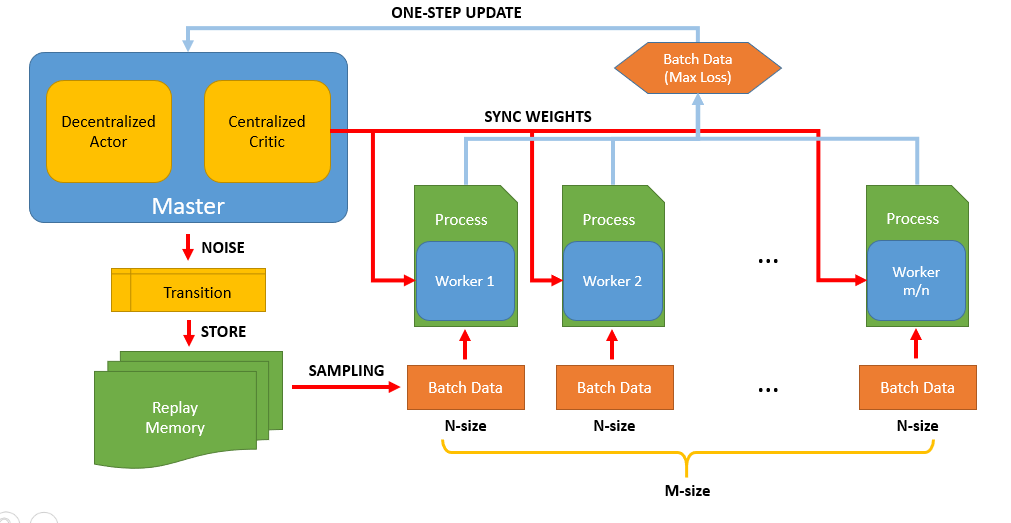
\includegraphics[width=12cm]{imgs/architecture.PNG}
  \caption{architecture}
  \label{fig:architecture}
 \end{center}
\end{figure*}

Recently, OpenAI rleased a method which extends traditional DDPG method to multi-agent domain \cite{maddpg}. As we know, single-agent algorithm failed because while agent is updating policy, the environment becomes non-stationary which turns out to failure of convergence. Multi-Agent DDPG, in Fg.\ref{fig:maddpg} found a centralized way to put other agents's actions into consideration in critic.
\begin{equation}
L(\theta_i) = E_{s,a,r,s'}[y - Q(s, a_1, a_2 ... a_n)],  
\end{equation}
$$where\ y = r_i + \gamma{Q_i}(s', a_1', a_2' ... a_n') | _{a_j'=\mu_j'(o_j)}$$

MADDPG is a great algorithm which uses centrilized critic to take other agents' actions into consideration, it turns out to be a stable learning method compared with traditional RL methods. \par

MADDPG still uses experience replay, which is same as in DDPG, to stablize the learning process. Experience replay \cite{replay} memory can store transitions of the form $(s,a,r,s')$, and agent can sample batches to do updates. The sampling process breaks the correlation between transitions and improves learning's stability. \par

However, multi-agent setting has tremendous situations comparing with single-agent setting, the experiment replay memory from single multi-agent system may seem not enough for learning. Also, different batches from sampling could have a totally different effect on learning, which means it will be great for us to select good batches for updates to accelerate and improve learning process. \par

In this work, I present a distributed multi-worker architecture for batch data collection and a sellection method for prioritized batch data.


\subsection{Distributed Multi-Agent architecture}

First, in order to collect batch data (transitions) effciently, we use asynchronous workers, similarly to Asynchronous RL Framework \cite{a3c}, but instead of using multi-thread, we use multi-process on a single machine. And we use MPI (Message Passing Interface) for data transfer among processes. Each worker on each process is able to asychronously run its own environment and collect batch data and sychronously send data to master (the main process for learning) and recieving nerual network weights from the master. \par

Second, multiple workers running in parallel with different random seed is likely to explore different situations of the same environment. Moreover, exploration noise in different parallel world could attribute to the exploration's diversity. \par

\subsection{Prioritized Batch Data}

Experience replay addresses the following issues: it helps to break the temporal correlations by sampling from big fixed-size memory. What measures batch data as good one or bad one it how much it could lead to a better single update. Temporal-Difference error (TD error) used in DDPG is the difference between target network Q value and evalution network Q value. The bigger TD error is, the better this update is. \par

To select good batch data for updating, we could firstly sample a $M$ (bigger size) batches, we plan to select $N$ (smaller size) batches for update. We divide $M$ size batches into $M/N$ size parts, we calculate each part's loss. We choose the part of batches with biggest loss to train. We call these good batch data as Prioritized Batch Data. \par

For example, $M = 256$ and $N = 64$, we first sample $256$ batches from experience replay. Because $M / N = 4$, we divide $256$ batches into $4$ parts, and calculate loss for each part. If the result is {$11.1, 10.5, 30.2, 4.1$}, we know the third part has biggest loss, so we choose third part of batch data to do updating. 

\section{Experiments}
In this section, we will introduce the experiment environment we use and several experiments we carried to verify the superiority of our proposed method.

\subsection{Experiment Environment}
To perform our experiments, we adopt the multiagent-particle-envs used in \cite{maddpg}, which consists of $N$ agents and $L$ landmarks inhabiting a two-dimensional world with continunous observation space and continunous action space. There are several types of environment it provides with. We focus on multi-agent cooperation for chasing target, so we adopt Predator-Prey environment.\par
In this Predator-Prey environment, $N$ slower cooperating agents try to chase the faster target which could flee away from chasers around a randomly generated environment with $L$ large landmarks served as obstacles to blcok the way. Each time agents collide with a target, the agens are rewarded while the target is penalized. \par
Due to being short of calculation capability and resources, we add some constrains in Predator-Prey environment.
\begin{itemize}
  \item $N$ Predators, $\in$ $[2, 4]$ with random initial position.
  \item $M$ Preys, $\in$ $[1, 2]$ with random initial position.
  \item $1$ Landmark, with a fixed position in middle.
\end{itemize}
The action space is Box(5) in gym \cite{gym}
\begin{table}[ht]
 \caption{action space} 
 \label{tbl:action}
  \begin{center}
    \begin{tabular}{c|ccc}
  Num  & Action & Min & Max\\
  \hline \hline
  0 & No use &  & \\
  1 & Power toward right & -1.0 & 1.0\\
  2 & Power toward left & -1.0 & 1.0\\
  3 & Power toward up & -1.0 & 1.0\\
  4 & Power toward down & -1.0 & 1.0\\\hline
    \end{tabular}
  \end{center}
\end{table}
Rewards for predators
\begin{itemize}
  \item +10 points, any one agent of predators collides with one of preys
  \item -0.1 * distance points, decreased reward for increased distance from agents
\end{itemize}

Rewards for preys
\begin{itemize}
  \item - 10 points, when prey itself collides with predators
\end{itemize}

The observation space is Box($6+N*2$) for each chaser and Box($4+N*2$) for target, which includes every agent's position and environment information.



\subsection{Network Architecure}
In order to have proper hyperparameters and network, we get ideas from \cite{param} and use the following settings.

\begin{table}[ht]
 \caption{Hyper Parameters} 
 \label{tbl:hyperparameters}
  \begin{center}
    \begin{tabular}{c|ccc}
  \hline \hline
  Actor Learning rate  & 0.001   \\
  Critic Learning rate & 0.01    \\
  Gamma                & 0.99    \\
  Replay memory size   & 1000000 \\
  Minibatch size       & 64      \\
  Max episodes         & 10000   \\
  Max episode length   & 200     \\
  Random seed          & 1234    \\\hline
    \end{tabular}
  \end{center}
\end{table}

We use 2 hidden layers with 400 and 300 units in our network.
Each layer uses ReLU activation function to keep good information.
For actor, we use tanh to keep value between $[-1, 1]$. 

\subsection{Results}

\begin{figure}[ht]
 \begin{center}
  \includegraphics[width=7cm]{imgs/2vs1_maddpg_prioritized_result.png}
  \caption{DMADDPG, MADDPG, DDPG (2 vs 1)}
  \label{fig:result1}
 \end{center}
\end{figure}

DMADDPG is best.

\begin{figure}[ht]
 \begin{center}
  \includegraphics[width=7cm]{imgs/2vs1_maddpg_prioritized_result.png}
  \caption{DMADDPG, MADDPG, DDPG (4 vs 2)}
  \label{fig:result1}
 \end{center}
\end{figure}

DMADDPG is best.

\begin{table}[ht]
 \caption{Total rewards of 200 episodes} 
 \label{tbl:reward}
  \begin{center}
    \begin{tabular}{|c|c|c|}
    \hline
    Algorithm  & 2 vs 1 & 4 vs 2 \\
    \hline \hline
    DDPG vs DDPG     & 200 & 400  \\\hline
    MADDPG vs DDPG   & 400 & 1000 \\\hline
    DMADDPG vs DDPG  & 600 & 3000 \\\hline
    \end{tabular}
  \end{center}
\end{table}
DMADDPG is best.

\section{Conclusion}
In this work, there are two problems in multi-agent task, one is that traditional RL methods can't solve multi-agent task because environment becomes non-stationary during learning and leanring cannot converge, the second one is that random sampling batch data from experience replay is effcient for learning. We explain our proposed method - Distributed Multi-Agent Cooperation Algorithm besed on MADDPG algorithm using prioritized batch data in solving Predator-Prey task. Experiments shows we have xx\% faster convergence and xx times rewards comparing to MADDPG and DDPG.
Hyperparameters tuning and network architecture choice still remain a lot of work to fix.
And due to current limited hardward resources, our experiment cost a lot time. This will be improved in future.

\begin{comment}

\section{序論}
執筆要領について述べる。

\subsection{用紙}
A4用紙を縦長に使用する。本文は8ページ(表裏で4枚)以上、24ページ以内を標準とする。

\subsection{ヘッダ・フッタ}
ヘッダの左側には、「筑波大学大学院博士課程システム情報工学研究科修士論文」につづけて、修了年度・月を括弧書きで記述する。
ヘッダの右側には、氏名を記述する。氏名については、見やすくするために適宜空白をいれても差し支えない。

フッタの中央には、ページ番号をハイフンはさんで記述する。

\subsection{1ページ目の体裁}
申請する学位(修士(工学))を四角囲みで記述し、
つづけて修士論文のタイトルをそれぞれ日英表記で記述する。
ただし本文が英文の場合、英日の順に記述する。

つぎに、氏名・所属専攻と指導教員名・指導教員の所属を日英表記で記述する。
氏名・指導教員名については、見やすくするために適宜空白をいれても差し支えない。
ただし本文が英文の場合、英日の順に記述する。


\subsection{要約・キーワード}
修士論文の概要を記述する。
本文が日本語・英語に係らず概要は英語で記述する。


\subsection{本文}
本文は2段組みとし、10.5pで記述する。
句読点は、各分野で用いられる記号を使用する。

\subsection{図表}
論文として印刷に耐えうる品質(解像度)の図表を作成する。
図表中、および、キャプションは、原則として英語を使用する。
キャプションは、図の下と表の上に挿入する。
図番号および表番号は、それぞれ Figure 1、Table 1 のように表記する。
横長の図・表の場合は、段抜きで挿入してもよい。

たとえば、Figure \ref{fig:samplefigure}や Table \ref{tbl:sampletable}を例として示す。

\begin{figure}[t]
 \begin{center}
  \includegraphics{sample.eps}
  \caption{Sample figure}\label{fig:samplefigure}
 \end{center}
\end{figure}

\begin{table}
 \caption{Sample table} \label{tbl:sampletable}
\begin{center}
  \begin{tabular}{c|ccc}
  A & B & C & D\\
  \hline \hline
  a & b & c & d\\
  a & b & c & d\\ \hline
 \end{tabular}
\end{center}
\end{table}

\subsection{数式}
数式のサンプルとして、(\ref{eq:gauss})を示す。
\begin{equation}
 \int _\infty ^\infty e^{-x^2}dx = \sqrt{\pi} \label{eq:gauss}
\end{equation}

\subsection{参考文献}
それぞれの分野の記述法により、十分な数の参考文献を引用する\cite{osamu}。著者が執筆した修士論文に関連する内容の論文等がある場合には、必ず文献として引用する。

\subsection{著者紹介}
学会誌論文の一般的な著者紹介を例に記述する。

\subsection{付録}
本文には書ききれないデータなどは、
付録に収めることができる。付録は、研究室で別途保管する。



\section{\LaTeX スタイルファイルについて}
このサンプルは、筑波大学大学院システム情報工学研究科知能機能システム専攻の修士論文を\LaTeX で作成するためのスタイルファイルである。
配布ファイルは以下の通りである。
\begin{description}
 \item[iit-jp-sjis.sty]  知能機能システム専攻の修士論文のためのスタイルファイル
 \item[templete.tex] スタイルファイルを利用するためのテンプレートファイル
 \item[face.eps] 顔写真用のテスト画像
 \item[sample.eps] Figure のためのテスト画像
\end{description}

スタイルファイルやテンプレートは、適宜改良をして使用してもよい。

\section*{謝辞}
本研究は、・・・・・・深謝する。


%\addcontentsline{toc}{section}{\numberline{}参考文献}

\begin{thebibliography}{9}
\bibitem{osamu}  工学修得, ``修士論文の書き方'', 知能機能システム学会論文誌, Vol.1, No.2, pp.34--56, 2015.
\end{thebibliography}


\vspace{2zh}
\begin{minipage}{73mm}
 \begin{wrapfigure}[6]{l}[-4pt]{30mm} 
 \begin{center}
  \includegraphics[width=30mm]{face.eps}
 \end{center}
 \end{wrapfigure}
 \noindent 筑 \ 波 \ 太 \  郎\\\\
 筑波大学大学院システム情報工学研究科知能機能システム専攻所属
\end{minipage}

\vspace{3zh}
----------------------------------------------\par

\begin{itemize}
 \item Webで公開する論文の概要は、別に作成する。
 \item 修士論文は両面印刷とする。
 \item 修士論文提出時は、ソフトカバーを施して必要部数を大学院教務に提出する。背表紙は不要。
 \item 論文審査後に、両面印刷したもの(綴じていないもの)を専攻長に提出する。
 \item 専攻長は、専攻全員の修士論文をハードカバーにて製本し、専攻室で保管する。
\end{itemize}

\begin{itemize}
 \item Extended summary is also required for uploading onto the web.
 \item The thesis should be printed in double face printing.
 \item Submit your thesis to the academic service office. The thesis should be clapped with a soft-cover.
 \item  Submit your thesis to the chair of the iit, after it has passed the examining meeting. The thesis should not be clapped.
 \item The chair of the iit will bind up all the accepted theses and preserve in his/her office.
\end{itemize}
https://scholar.google.com/scholar?hl=zh-CN&as_sdt=02C5&q=policy+gradient&btnG=
\end{comment}

\addcontentsline{toc}{section}{\numberline{}References}

\begin{thebibliography}{9}

\bibitem{alphago}
David Silver, Aja Huang, et al. Mastering the Game of Go with Deep Neural Networks and Tree Search. Nature, 529(7587):484–489, 2016.

\bibitem{alphagozero} 
David Silver, Julian Schrittwieser, et al. Mastering the game of Go without human knowledge. Nature, 550:354–359, 2017.

\bibitem{starcraft} 
DeepMind and Blizzard open StarCraft II as an AI research environment. https://deepmind.com/blog/deepmind-and-blizzard-open-starcraft-ii-ai-research-environment.

\bibitem{game}
 P. Peng, Q. Yuan, et al. \textsl{Multiagent bidirectionally-coordinated nets for learning to play starcraft combat games}. CoRR, abs/1703.10069, 2017.

\bibitem{robot}
L. Matignon, L. Jeanpierre, A.-I. Mouaddib, et al. \textsl{Coordinated multi-robot exploration under
communication constraints using decentralized markov decision processes}. In AAAI, 2012.

\bibitem{google}
DeepMind AI reduces google data centre cooling bill by 40. https://deepmind.com/blog/deepmind-ai-reduces-google-data-centre-cooling-bill-40/.

\bibitem{maddpg} 
R Lowe, Y Wu, A Tamar, et al. \textsl{Multi-Agent Actor-Critic for Mixed Cooperative-Competitive Environments}.arXiv:1706.02275v2, 2017.

\bibitem{cover-heuristic}
A Isaza, J Lu, et al. \textsl{A Cover-Based Approach to Multi-Agent Moving Target Pursuit}. AIIDE, 2008.

\bibitem{qlearning} 
Christopher JCH Watkins and Peter Dayan. \textsl{Q-Learning}. Machine Learning, 8(3-4):279–292, 1992.

\bibitem{pg} 
R. S. Sutton, D. A. McAllester, S. P. Singh, and Y. Mansour. \textsl{Policy gradient methods for rein-
forcement learning with function approximation}. In Advances in neural information processing systems, pages 1057–1063, 2000.

\bibitem{ddpg} 
Timothy P Lillicrap, Jonathan J Hunt, et al. \textsl{Continuous Control with Deep Reinforcement Learning}. In ICLR, 2016.

\bibitem{ppo} 
John Schulman, Filip Wolski, et al. \textsl{Proximal Policy Optimization Algorithms}.arXiv:1707.06347, 2017.

\bibitem{cover} 
Xiao Tang, Nobuhara Hajime. \textsl{Real-time Grid-based Multi-Agent Pursuing A Moving Target method}. the 79th national convention of IPSJ, 2016. 

\bibitem{dpg} 
David Silver, Guy Lever, et al. \textsl{Deterministic Policy Gradient Algorithms}. In ICML, 2014.

\bibitem{dqn} 
Volodymyr Mnih, Koray Kavukcuoglu, et al. \textsl{Human-Level Control through Deep Reinforcement Learning}. Nature, 518(7540):529–533, 2015.

\bibitem{replay} 
Long-Ji Lin. \textsl{Self-Improving Reactive Agents Based on Reinforcement Learning, Planning and Teaching}. Machine Learning, 8(3–4):293–321, 1992.

\bibitem{a3c} 
Volodymyr Mnih, Adria Puigdomenech Badia, et al. \textsl{Asynchronous Methods for Deep Reinforcement Learning}. In ICLR, 2016.

\bibitem{a2c} 
Jane X Wang, Zeb Kurth-Nelson, et al. \textsl{Learning to Reinforcement Learn}. In CogSci, 2017.

\bibitem{param}
Peter Henderson, Riashat Islam, et al. \textsl{Deep Reinforcement Learning that Matters}. arXiv:1709.06560, 2017.

\bibitem{gym}
https://github.com/openai/gym

\vspace{2zh}
\begin{minipage}{73mm}
 \begin{wrapfigure}[6]{l}[-4pt]{30mm} 
 \begin{center}
  \includegraphics[width=30mm]{face.eps}
 \end{center}
 \end{wrapfigure}
 \noindent 筑 \ 波 \ 太 \  郎\\\\
 筑波大学大学院システム情報工学研究科知能機能システム専攻所属
\end{minipage}

\end{thebibliography}
\clearpage
\section{Appendix}


\begin{algorithm*}[ht]
\caption{Distributed Multi-Agent DDPG algorithm (Master)}
\begin{algorithmic}
\State {Initialize replay memory $\mathbb{D}$}
\State {Initialize a random process $\mathbb{N}$ for action exploration}
\For {$episode = 1$ to max-episodes}
  \State {Recieve initial obsercation state $s$}
  \For {$t = 1$ to max-episode-length}
    \For {agent $i = 1$ to n}
      \State {Get prioritized batch data of N (${s_j, a_j, r_j, s_j'}$) from $\mathbb{D}$}
      \State {$y = r^i + Q^i_{\bar{\mu^i}}(o_j^i, a_j^1, a_j^2,\dots, a_j^i)|_{a_j^k=u^i(o_j^i)}$}
      \State {Update critic by minimizing the loss $L(\theta_i) = E_{s,a,r,s'}[(Q(s, a_1, a_2 ... a_n) - y)^2]$}
      \State {Update actor using the sampled policy gradient:
      $$
         \bigtriangledown_{\theta^\mu} J
          = \sum \bigtriangledown_{a}Q(s, a|\theta^\mu)\bigtriangledown_{\theta^\mu}\mu(s|\theta^\mu)
      $$
      }
    \EndFor
    \State {Update target network parameters for each agent i:
      $$\bar{\theta^i} \leftarrow \tau \theta^i + (1 - \tau)\bar{\theta^i}$$
    }
  \EndFor
  \State {Sychronouly get batch data from Workers and add it to replay memory $\mathbb{D}$}
  \State {Asychronously send network weights to each worker}
\EndFor
\end{algorithmic}
\end{algorithm*}

\begin{algorithm*}[ht]
\caption{Distributed Distributed Multi-Agent DDPG algorithm (Worker)}
\begin{algorithmic}
\State {Create actor, actor target, critic, critic target network for master and each worker}
\State {Initialize buffer $\mathbb{D}$}
\State {Initialize a random process $\mathbb{N}$ for action exploration}
\For {$episode = 1$ to max-episodes}
  \State {Recieve initial obsercation state $s$}
  \For {$t = 1$ to max-episode-length}
    \For {agent $i = 1$ to n}
      \State {Get action $a^i$ based on each policy}
    \EndFor
    \State {Get reward $r$ from environment by taking actions}
    \State {Store (${s, a, r, s'}$) into buffer $\mathbb{D}$}
  \EndFor
  \State {Asychronously send buffer to Master and clean buffer}
  \State {Sychronouly get network weights from Master and update}
\EndFor
\end{algorithmic}
\end{algorithm*}


\end{document}
